\documentclass[10pt,a4paper]{article}
\usepackage[T1]{fontenc}
\usepackage[utf8]{inputenc}
\usepackage[magyar]{babel}
\usepackage{graphicx}
\usepackage{subcaption}
\usepackage{float}
\usepackage{amsmath}
\usepackage{anysize}
\usepackage{bm}
\usepackage{physics}
\DeclareGraphicsExtensions{.pdf,.png,.jpg,.svg}
\linespread{1.3}
\numberwithin{equation}{subsection}
\numberwithin{figure}{section}
\bibliographystyle{plain}
\usepackage{hyperref}


\newcounter{nextsec}
\newcommand\nextsection{%
  \setcounter{nextsec}{\thesection}%
  \stepcounter{nextsec}%
  \thenextsec%
}

\setlength\parindent{20pt}

\title{}

\newlength{\figurewidth}
\setlength{\figurewidth}{5cm}

\newenvironment{bfigure}[1]{\begin{figure} [#1] \begin{bf}}{\end{bf} \end{figure}}
\newcommand{\icaption}[1]{\caption{\textit{\textmd {#1}}}}
\newcommand{\colorg}[1]{{\color{green}{#1}}}

\begin{document}

\pagestyle{empty}


\begin{titlepage}

\center

\textsc{\LARGE  Eötvös Loránd Tudományegyetem}\\[0.5cm]
\textsc{\LARGE Természettudományi Kar}\\[1.5cm]
\textsc{\LARGE Fizikai Intézet}\\[1.5cm]
\vspace{8mm}

{ \huge \bfseries Háromrészecske Bose-Einstein korrelációk vizsgálata}\\[0.4cm] % Title of your document
\vspace{8mm}

\begin{center}
\LARGE \textit{Bagoly Attila}\\
\Large \textit{Fizikus MSc}\\
\end{center}

\begin{center}
\LARGE Témavezető: \\
\LARGE \textit{Csanád Máté}\\
\Large \textit{ELTE TTK Atomfizikai tanszék}\\
\end{center}
\vspace{4mm}



\begin{figure}[H] 
\centerline{ 

\includegraphics[height=5cm]{pic/ELTE_logo.png} 
} 
\end{figure}
\vspace{5mm}
\begin{Large}
\textbf{2017%. május 22.
}
\end{Large}

\end{titlepage}

%\section*{Abstract}
%Bose-Einstein correlations of identical hadrons reveal information about hadron
%creation from the sQGP formed in ultrarelativistic heavy ion collisions. The
%measurement of three particle correlations may in particular shed light on
%hadron creation mechanisms beyond thermal/chaotic emission. In my work I'm measuring three pion correlations as a function of momentum
%differences within the triplets in RHIC PHENIX experiment. I analyzed the shape of these functions through the assumption
%of Levy sources and a proper treatment of the Coulomb interaction within the
%triplets. We determine Levy parameters scale ($R$), shape ($\alpha$) and three
%particle correlation strength ($\lambda_3$), where the latter, together with two
%particle correlation strength $\lambda_2$, encodes information about hadron
%creation mechanisms. From a consistent analysis of two- and three-particle
%correlation strength we are able to establish an experimental measure of the thermalization and coherence in the source.

\newpage
\tableofcontents

\clearpage
\pagestyle{plain}
\setcounter{page}{1}



\section{Bevezetés}

\subsection{Nagyenergiás nehézion-fizika}



A nehézion-fizikában nagy rendszámú atommagok közel fénysebességen való ütköztetésével próbálunk információt szerezni az elemi részecskék világáról. Az atommagokat közel fénysebességre gyorsítjuk elektromágneses terek segítségével (LHC, RHIC a két legnagyobb energiájú gyorsító). A labor-rendszerből nézve Lorentz-kontrahált atommagokat összeütköztetünk,  az ütközés során lejátszódnak bizonyos valószínűséggel ``kemény'' folyamatok amelyek során részecskezáporok (jet) keletkeznek, melyek hadronokból, leptonokból és fotonokból állnak. A kemény folyamatok jellemzője, hogy a jetek párokban keletkeznek, majd az impulzusmegmaradás miatt ellenkező irányba haladnak, az ütközések során a legvalószínűbb egy jet-pár keletkezése. Egy ütközés során nem csak kemény folyamatok zajlanak, hanem a ``lágy'' folyamatok is, melyek során a részecskék nem jetekben keletkeznek. Az ütköző atommagok tömegközépponti energiájának növelésével nő a kemény folyamatok valószínűsége, és csökken a lágy folyamatoké. Az ütközési pont köré épített detektorok segítségével mérjük a keletkező részecskék eloszlásait és különböző fizikai paramétereit. Ezen adatok segítségével próbálunk következtetni az ütközés után lezajló jelenségekre.

Az ütközések jellemzésére definiálni szoktuk az impakt paramétert, amely a középpontok távolságát jelenti. Az impakt paraméter alapján centralitás osztályokba rendezzük az ütközéseket, ezen osztályokat a centrálistól periférikus fele haladva százalékosan adunk meg.

Másik fontos fogalom a nukleáris módosulási faktor, amely segítségével az ütközés folyamatát tudjuk jellemezni. Az ütközés centralitását ismerve ki tudjuk számolni az ütközésben résztvevő nukleonok számát. A teljes folyamatot elképzelhetjük bináris ütközések összegeként, amennyiben feltesszük, hogy a protonok páronként ütköznek és egymástól függetlenül zajlanak az események. Független p+p ütközésekből ismerjük egy ilyen esemény során keletkező részecskék számát. Nehézion ütközések esetén ezt a számot megszorozzuk az ütközés bináris eseményeinek számával, így megkapjuk a keletkező részecskék számát. Azonban ezt a számot közvetlenül is meghatározhatjuk két nehézion összeütköztetésével, az előbbivel vett arányt nevezzük a nukleáris módosulási faktornak. Például Au+Au ütközés esetén, ha a keletkező részecskék száma $N_{{\rm Au}}$, bináris ütközések száma $N_{{\rm bin}}$ és p+p ütközések esetén a keletkező részecskék száma $N_{{\rm p}}$ akkor a nukleáris módosulási faktor a következőképpen néz ki:
\begin{large}
\begin{equation}
R_{\rm AA}=\frac{N_{\rm Au}}{N_{\rm bin}N_{\rm p}},
\label{eq:e1}
\end{equation}
\end{large}
ennek értékére  $R_{\rm AA}=1$ várunk, mivel az Au+Au ütközéseket úgy képzeljük el, hogy az ütközésben résztvevő protonok páronként ütköztek.  

\begin{center}
\begin{figure}[H]
\centering
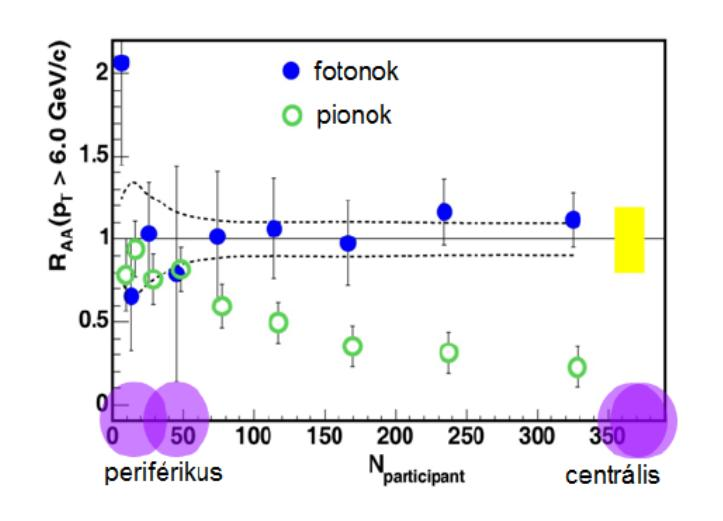
\includegraphics[scale=0.6]{pic/int/p1}
 \caption{Au+Au ütközések esetén a nukleáris módosulási faktor a nukleonszám függvényében pionokra és fotonokra. Az ábrán látható, hogy nagy centralitás esetén kevesebb nagyenergiás piont észlelünk mint p+p ütközések alapján várnánk, továbbá az erős kölcsönhatásban nem 
  fotonok száma a várttal egyezik. Ez utal az erősen kölcsönható közeg jelenlétére.}
\label{fig:mmf}
\end{figure}
\end{center}

\subsection{Kvark-gluon plazma}

A RHIC gyorsítóban Au+Au ütközések során nagy nagy centralitásnál mérések során kevesebb nagyenergiás részecskét mértek a p+p ütközések alapján vártnál (\ref{fig:mmf} ábra), a jet-párok egyik tagja nem jelent meg. Azonban ezen tapasztalatoknak több kiváltó oka is lehet, a kérdés eldöntésére további kísérleteket végeztek. Az egyik volt a deutérium-arany ütközések elvégzése, azonban itt semmilyen centralitásnál nem volt jet-elnyomás. Ennek magyarázata, hogy ütközések esetén erősen kölcsönható közeg jöhet létre amely a jet-pár egyik tagját elnyeli (amely nagyobb utat tesz meg benne), azonban deutérium-arany ütközések során a létrejövő közeg mérete túl kicsi, hogy elnyelje azt.

Ezen közeg létrejöttét elméletileg a QCD magyarázza meg. Az elmélet szerint nagyon nagy energián megjelennek kvark szabadsági fokok, azaz a kvarkok hadronba zártsága megszűnik. A létrejövő közeg az erősen kölcsönható kvark-gluon plazma nevet viseli (sQGP). Ezen közegben nagyok a hatáskeresztmetszetek, ezért kicsi a szabad úthossz és gyors a termalizáció, ezért van értelme lokális egyensúlyról beszélni, így alkalmazhatóak rá a statisztikus fizika fogalmai (pl. hőmérséklet). Az ősrobbanást követő egy milliomod másodpercben az univerzumot is a kvark-gluon plazma alkotta ~\cite{SWeinberg}.

Az új közeg felfedezése után a RHIC gyorsítóban ezen közeg tulajdonságainak megismerését célzó kísérletek kezdődtek. Ezen kísérletek során kiderült, hogy a kvark-gluon plazma az eddig látott legtökéletesebb (viszkozitás mentes) folyadékként viselkedik, amely meglepő volt hisz nagyon kis viszkozitással rendelkező folyadékokat eddig nagyon alacsony hőmérsékleten tudtak csak előállítani. A kvarkfolyadék viszkozitására a gravitációs- és kvantumtérelméletek analógiájából (AdS/CFT) származik egy alsó becslés, eszerint a viszkozitás nem lehet kisebb mint $\hbar/4\pi$.

\begin{center}
\begin{figure}[H]
\centering
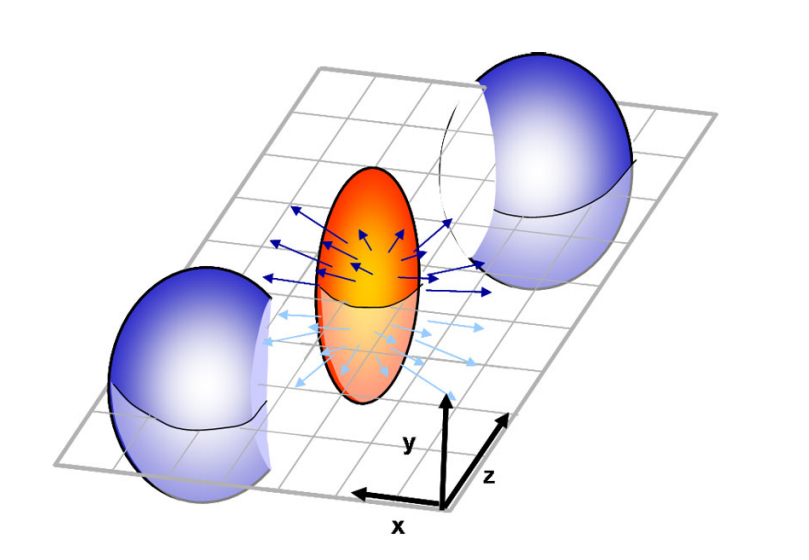
\includegraphics[scale=0.6]{pic/int/p2}
\caption{Két gömb ütközéseként létrejövő speciális ellipszoidális szimmetriával rendelkező kezdeti eloszlás kialakulása.}
\label{fig:ellip}
\end{figure}
\end{center}



Ultrarelativisztikus sebességre felgyorsított atommagok ütközése két Lorentz-kontrahált korong ütközéseként fogható fel, laborrendszerből nézve. Amint \aref{fig:ellip} ábra is szemlélteti, ez a létrejövő kvarkanyagban speciális kezdeti eloszlást eredményez, egy $\cos(2\varphi)$-szerinti aszimmetriát az eloszlásban, amely a tengelyszimmetriától való elliptikus eltérést jelenti.
A nyalábirányra merőlegesen bevezetjük a transzverz-síkot, ebben a síkban az kvarkanyag kezdeti eloszlását Fourier-sorba fejtjük a következőképpen:
\begin{large}
\begin{equation}
A(\varphi)= a_0+\sum_{n=1}^{\infty}\Big[a_n \cos(n\varphi)+b_n \sin(n\varphi)\Big]
\label{eq:e2}
\end{equation}
\end{large}
Ezen sorfejtés alapján látható, hogy az $a_2$ jellemzi az előbb említett aszimmetriát, amennyiben tökéletesen gömbszimmetrikusak lennének az atommagok és a keletkező ellipszis egyik nagytengelyén vennénk föl a a koordináta-rendszer x-tengelyét csupán ez a tag jelenne meg. Azonban mivel az atommagok véges nukleonszámmal rendelkeznek, melyeknek van valamilyen eloszlása a magon belül, a gömbszimmetria csupán első közelítésként fogható fel.

Az ütközés után létrejövő kvarkanyag robbanásszerűen tágul egész addig amíg a hőmérséklet le nem csökken egy bizonyos értékre, ekkor megszűnik ez a fázis és a kvarkokból hadronok keletkeznek amelyeket mérni is tudunk. Mivel a kvarkanyag folyadékszerűen viselkedik a kezdeti aszimmetriák nem tűnnek el, a kifagyás pillanatába is jelen vannak, ezért azok a keletkező hadronok eloszlásában is megjelennek. Az aszimmetriákat jellemző paramétereket az impulzustérben szokás definiálni. A részecskék eloszlását transzverz-síkban a $N(p_t, \varphi)$ függvénnyel jellemezzük, amely megmondja, hogy $[\varphi, \varphi+d\varphi]$ irányban $[p_t, p_t+dp_t]$ impulzus-tartományban mennyi részecske található. A függvény szögfüggését leválasztva, azt Fourier-sorba fejtve és 1-re normálva a következő alakban írhatjuk:
 \begin{large}
\begin{equation}
N(p_t, \varphi)= N(p_t)\bigg(1+\sum_{n=1}^{\infty}\Big[v_n \cos(n\varphi)+w_n \sin(n\varphi)\Big]\bigg)
\label{eq:e3}
\end{equation}
\end{large}
A Fourier-sor első komponensei játszanak fontosabb szerepet. Ezek közül is a $v_2$ együttható a leglényegesebb, mert ez a paraméter hordozza az ellipszoidális aszimmetriát, ezt az elliptikus folyás paraméterének nevezzük. Ezen aszimmetria a kifagyott hadronok és fotonok eloszlásában ~\cite{Adare:2011zr} is megjelenik, ezért a folyadékkép helyességét bizonyítja a kvark-gluon plazma esetén.
A Fourier-sor szinuszos részét nem szoktuk külön kezelni, mivel a mérések során a reakciósíkhoz képesti szög szerinti sort veszünk ($\sum v_n \cos[n(\varphi-\psi_n)])$, így a fenti szinuszos és koszinuszos tagok összevonva jelennek meg. Más mérési módszer esetén ugyan megjelenhetnek külön is a szinuszos tagok, de ekkor is szimmetria okokból ezen tagok eltűnnek.


\subsection{A PHENIX kísérlet}



\section{Bose-Einstein korrelációk}

Bose-Einstein korrelációk vizsgálatának megalapozói Robert Hanbury Brown és Richard Q. Twiss volt, ők 1956-ban publikált cikkükben ~\cite{HanburyBrown:1956bqd} vezették be a módszert, azonban munkájuk vegyes fogadtatásban részesült a tudományos közösség részéről. A módszert segítségével képesek voltak meghatározni a Sirius csillag átmérőjét a fotonok közötti korrelációk méréséből. Mérési elrendezésük két változtatható távolságra levő foton detektorból állt (ezek egy-egy fókuszáló tányér és fotoelektron-sokszorozóból álltak). A két detektor segítségével mérték a Sirius csillagból jövő fotonok közti korrelációt, különböző detektortávolságokon. Az így kapott pontokra elméleti megfontolásokból kapott korrelációs függvényt illesztettek, amely segítségével meghatározták a csillag átmérőjét. A két tudós tiszteletére a bozonok közti intenzitás korrelációt szokás Hanbury Brown és Twiss effektusnak nevezni (vagy röviden HBT effektus), az ilyen jellegű vizsgálódásokat pedig HBT analízisnek.

A HBT effektus részecskefizikai alkalmazásában jelentős szerepet játszott G. Goldhaber, S. Goldhaber, W.Y. Lee és A. Pais kutatása, akik proton-antiproton $1.05\;\mathrm{GeV/c}$ tömegközépponti energián történő ütköztetésekben keletkező pionokat vizsgáltak. Mérésük során azonos pionok között nem várt korrelációt tapasztaltak, melynek vizsgálatával felfedezték a $\rho^0$ rezonanciát, amely $4.5\cdot 10^{-24}$ másodperc alatt elbomlik két pionra ($\rho^0\rightarrow \pi^+\pi^-$), eredményüket 1960-ban publikálták ~\cite{Goldhaber:1960sf}. Később kiderült, hogy az általuk tapasztalt korrelációnak az oka, hogy a fotonokhoz hasonlóan a pionok is bozonok. Goldhaber és társai kutatása nyomán a részecskefizikában is beindult a HBT effektus vizsgálata. Későbbiekben kiderült, hogy az asztrofizikához hasonlóan ezek a korrelációk itt is információt hordoznak a forrás geometriájáról ~\cite{Padula:2004ba}. 


\subsection{Definíció}

Általánosan n részecske közti korrelációs függvény a következőképpen definiálható ~\cite{Alt:1999cs, Csorgo:1999sj}:
\begin{equation}
C_n(p_1, p_2, \dots, p_n)=\frac{ N_n(p_1, p_2, \dots, p_n)  }{ N_1(p_1)N_1(p_2)\dots N_1(p_n)},
\label{eq:Cn}
\end{equation}
ahol $p_i=(p_i^0, \bm{p_i})$ 4-es impulzusmomentum, $ N_n(p_1, p_2, \dots, p_n)$ az n részecske invariáns momentum eloszlás. A korrelációs függvény szemléletesen azt mondja meg, hogy milyen valószínűséggel keletkezik egy részecske n-es $p_1, p_2, \dots, p_n$ 4-es momentumokkal.

Az n részecske invariáns impulzusmomentum eloszlás meghatározható a következő módon:
\begin{equation}
N_n(p_1, p_2, \dots, p_n) = \int \prod_{i=1}^{n}\mathcal{S}(p_i, x_i)\abs{\Psi_{p_1, {p_2}, \dots, {p_n}}({x_1}, {x_2}, \dots, {x_n})}^2\prod_{i=1}^{n}d^4 x_i,
\label{eq:Nn}
\end{equation}
ahol a $\Psi_{p_1, {p_2}, \dots, {p_n}}({x_1}, {x_2}, \dots, {x_n})$ az n részecske hullámfüggvény, az $\mathcal{S}({p_i}, {x_i})$ pedig az úgynevezett forrásfüggvény, amely megadja annak a valószínűségét, hogy ${x_i}$ helyen keletkezik egy részecske ${p_i}$ impulzussal.

Az n részecske hullámfüggvény meghatározásához nemrelativisztikus közelítést használunk HBT effektus vizsgálata során, így a függvényt a Schrödinger egyenlet megoldásából kapjuk (ügyelve, arra hogy mivel bozonjaink vannak, két részecske felcserélésére szimmetrikus legyen a hullámfüggvény):
\begin{equation}
i\hbar\frac{\partial \Psi(\bm{x_1},\dots, \bm{x_n},t )}{\partial t} = \Bigg[\sum_{i=1}^{n}\bigg(-\frac{\hbar^2}{2m_i}\Delta_i + V_i(\bm{x_i})\bigg) + \frac{1}{2}\sum_{i\neq j} V_{ij}(\bm{x_i},\bm{x_j})\Bigg]\Psi(\bm{x_1},\dots, \bm{x_n} ,t)
\label{eq:Sch0}
\end{equation}

A HBT effektus vizsgálatánál a különböző számítások könnyítése érdekében elhanyagoljuk az erős kölcsönhatást, amely tapasztalatok szerint pionok esetén megtehető, de már protonok esetén nem ~\cite{Pratt:1990zq}. Továbbá csak a párok közti Coulomb-kölcsönhatást vesszük figyelembe, elhanyagolva többi hadron által okozott töltésfelhőt. Így ~\aref{eq:Sch0} egyenlet a következő, egyszerűbb alakra egyszerűsödik:
\begin{equation}
i\hbar\frac{\partial \Psi(\bm{x_1},\dots, \bm{x_n},t )}{\partial t} = \Bigg[-\sum_{i=1}^{n}\frac{\hbar^2}{2m_i}\Delta_i + \frac{1}{2}\sum_{i\neq j} V_C(\bm{x_i},\bm{x_j})\Bigg]\Psi(\bm{x_1},\dots, \bm{x_n} ,t)
\label{eq:Sch}
\end{equation}

Mivel energia saját állapotokkal dolgozunk, ezért  ~\aref{eq:Sch} egyenletet megoldó hullámfüggvény felírható:
\begin{equation}
\Psi_{p_1, {p_2}, \dots, {p_n}}(\bm{x_1},\dots, \bm{x_n},t )  
= \Psi_{\bm{p_1}, \bm{p_2}, \dots, \bm{p_n}}(\bm{x_1}, \bm{x_2}, \dots, \bm{x_n})\prod_{i=1}^ne^{-\frac{i}{\hbar}cp_i^0t},
\end{equation}
ahol $\Psi_{\bm{p_1}, \bm{p_2}, \dots, \bm{p_n}}(\bm{x_1}, \bm{x_2}, \dots, \bm{x_n})$ az időfüggetlen Schrödinger egyenlet megoldása:

\begin{equation}
\Bigg[-\sum_{i=1}^{n}\frac{\hbar^2}{2m_i}\Delta_i + \frac{1}{2}\sum_{i\neq j} V_C(\bm{x_i},\bm{x_j})  
 - c\sum_{i=1}^n p_i^0
 \Bigg]\Psi_{\bm{p_1}, \bm{p_2}, \dots, \bm{p_n}}(\bm{x_1}, \bm{x_2}, \dots, \bm{x_n}) = 0
\end{equation}

Továbbá könnyedén belátható, hogy ~\aref{eq:Nn} egyenletben szereplő hullámfüggvény abszolút értéke szimmetrizációt elvégezve a következő lesz  (nemrelativisztikus közelítésben mondhatjuk, hogy $\bm{x_i} = (t,\bm{x_i})$) :
\begin{equation}
\abs{\Psi_{{p_1},{p_2}, \dots,{p_n}}({x_1}, {x_2}, \dots, {x_n})} = \frac{1}{\sqrt{n}}\abs{\sum_{(\alpha)}\Psi_{\bm{p_1}, \bm{p_2}, \dots, \bm{p_n}}(\bm{x_{\alpha_1}}, \bm{x_{\alpha_2}}, \dots, \bm{x_{\alpha_n}})}
\label{eq:Psin}
\end{equation}
ahol $\sum_{(\alpha)}$ az $(1,2,\dots,n)$ összes permutációjára való összegzés.


\subsection{Két nem kölcsönható részecske korrelációs függvénye}

Két azonos részecske esetén, nem kölcsönható esetben ~\aref{eq:Sch} egyenlet könnyedén megoldható, megoldásai a jól
ismert síkhullámok. A kétrészecskés invariáns impulzuseloszlásban szereplő hullámfüggvény szimmetrizáció
elvégzése után a következő lesz:
\begin{equation}
\Psi_{{p_1}{p_2}({x_1},{x_2})} = \frac{1}{\sqrt{2}}\big({e^{{ip_1x_1}+i{p_2x_2}}+e^{i{p_2x_1}+i{p_1x_2}}}\big)
\end{equation}

A ${K}={p_1+p_2}$, ${k}=\frac{{p_1-p_2}}{2}$, ${r}={x_1-x_2}$, ${R}=\frac{{x_1+x_2}}{2}$ változókra áttérve (ezen transzformáció esetén az integrálási mérték nem változik, hiszen $d^4x_1d^4x_2=d^4Rd^4r$) a hullámfüggvény abszolút értéke a következő alakra egyszerűsödik:
\begin{equation}
\abs{\Psi_{{p_1}{p_2}}({r},{R})} = \frac{1}{\sqrt{2}}\abs{e^{{KR}}(e^{i{kr}}+e^{-i{kr}})}=\sqrt{2}\abs{\cos{2{kr}}}
\end{equation}

Ebből következőleg a kétrészecske invariáns momentumeloszlásra a következő alak adódik):
\begin{equation}
N_2({p_1},{p_2})=\tilde{\mathcal{S}}(0, {p_1})\tilde{\mathcal{S}}(0, {p_2})+\frac{1}{2}\big(\tilde{\mathcal{S}}(2{k}, {p_1})\tilde{\mathcal{S^*}}(2{k}, {p_2})+\tilde{\mathcal{S^*}}(2{k},{ p_1})\tilde{\mathcal{S}}(2{k}, {p_2})\big),
\end{equation}

ahol $\tilde{\mathcal{S}}$ a forrásfüggvény Fourier transzformáltja:
\begin{equation}
\tilde{\mathcal{S}}({q}, {k})=\int d^4x\mathcal{S}(x,k)e^{i{qx}}
\end{equation}

Az egyrészecske invariáns momentumeloszlásra pedig $N_1({p})=\tilde{\mathcal{S}}(0, {p})$ adódik. Ezekből ~\aref{eq:Cn} definíciót használva a kétrészecske korrelációs függvényre kapjuk a következő alakot:

\begin{equation}
C_2({p_1},{p_2}) = 1+ \frac{\tilde{\mathcal{S}}(2{k}, {p_1})\tilde{\mathcal{S^*}}(2{k}, {p_2})+\tilde{\mathcal{S^*}}(2\bm{k},{ p_1})\tilde{\mathcal{S}}(2\bm{k}, {p_2})}{2\tilde{\mathcal{S}}(0, {p_1})\tilde{\mathcal{S}}(0, {p_2})}
\end{equation}

Szokás alkalmazni a ${p_1}\approx {p_2}\approx {K} = p_1+p_2$ közelítést ($q\ll K$), amelyet az indokol, hogy a  forrást Fourier transzformáltjának az egyes részecskék momentumától való függése sokkal simább mint a relatív momentumtól való függése ~\cite{Lisa:2005dd}. A kétrészecske korrelációs függvény ekkor: 
\begin{equation}
C_2({k}, {K})=1+\frac{\abs{\tilde{\mathcal{S}}(2{k},{K})}^2}{\abs{\tilde{\mathcal{S}}(0,{K})}^2}
\end{equation}

Ez az alak azt a fontos üzenetet hordozza, hogy a kétrészecske korrelációs függvény meghatározásával megkapjuk a forrásfüggvény Fourier transzformáltját. Tehát a korrelációs függvény méréssel a forrás függvényt meg tudjuk határozni. 


A korrelációs függvény a $k,K$ négyes impulzusok helyett hármas momentumokkal is kifejezhető, ugyanis a két négyesmomentum szorzata definíció és az egyes részecskék tömeghéj feltétele ($p_{i\mu}p^{\mu}_i=0$) alapján eltűnik, azaz:
\begin{equation}
0=kK=k_0K_0-\bm{kK}\Rightarrow k_0 = \frac{\bm{kK}}{K_0}
\end{equation}

A $p_1\approx p_2\approx K$ feltevés alapján a $K$ körülbelül tömeghéjon van, azaz $K_0 = \sqrt{m^2-\bm{K}^2}$, így a korrelációs függvény a $k,K$ négyes-momentumok helyett a $\bm{k},\bm{K}$ hármas-momentumok függvényeként is tekinthető.

\subsection{Forrás függvény}
~\Aref{eq:Nn} egyenletben szereplő $\mathcal{S}({p},{x})$ függvényt nevezzük forrásfüggvénynek, ez megadja annak a valószínűségét, hogy ${x}$ helyen keletkezik egy ${p}$ impulzusú részecske. Az általunk vizsgált energiákon, az ütközés során kvark-gluon plazma keletkezik, amely robbanásszerűen tágul, melynek következtében csökken a hőmérséklete. Ha lokálisan a QGP elér egy bizonyos hőmérsékletet, akkor fázisátmenet történik, kifagynak a kvark szabadsági fokok és hadronok keletkeznek. A forrásfüggvényt épp ezen fázisátmenetek határozzák meg. 

A fázisátmenetet pillanatszerűnek tekinthetjük, mivel ha feltesszük, hogy ez nem teljesül, akkor mondhatjuk, hogy a forrásfüggvény felírható szorzat alakban: $\mathcal{S}({x}) = \mathcal{S}_T(\tau)\mathcal{S}(\bm{x})$. Az időfüggő részre feltehető továbbá:
\begin{equation}
\mathcal{S}_T(\tau)=\frac{1}{(2\pi \Delta\tau)^\frac{3}{2}}e^{-\frac{(\tau-\tau_0)^2}{2\Delta\tau^2}}
\end{equation}

Térszerű részre kevés megszorítással élve, a kétrészecske korrelációs függvényre a következő alak adódik:
\begin{equation}
C_2(k)=1+\lambda e^{-k_0\Delta\tau^2-k_{\mathrm{long}}R_{\mathrm{long}}^2-k_{\mathrm{side}}R_{\mathrm{side}}^2-k_{\mathrm{out}}R_{\mathrm{out}}^2},
\end{equation}
ahol az $R_{\mathrm{long}},R_{\mathrm{side}},R_{\mathrm{out}}$ az úgynevezett HBT sugarak. Továbbá adódik a HBT sugarak közti következő összefüggés:
\begin{equation}
R_{\mathrm{out}}^2-R_{\mathrm{side}}^2\propto \Delta\tau^2
\end{equation}

Kísérleti tapasztalat továbbá, hogy $R_{\mathrm{out}}\approx R_{\mathrm{side}}$, ebből következőleg a $\Delta\tau\approx 0$, tehát, a  forrásfüggvény időfüggő része egy $\tau_0$-ra koncentrált Dirac-delta, azaz a fázisátmenet pillanatszerűen történik ~\cite{Ster:2010ia, Csorgo:1999sj, Csanad:2009wc}.

%~\Aref{eq:Psin} egyenletnél láttuk, hogy az invariáns momentum eloszlásban megjelenő hullámfüggvény időfüggetlen.


A forrásfüggvény alakjára elsődlegesen Gauss eloszlást alkalmaztak ~\cite{Csorgo:2005gd, Lisa:2005dd}, azonban a PHENIX kísérletben $\sqrt{s_{NN}}=200\;\mathrm{GeV}$ tömegközépponti energiájú arany-arany ütközések során bizonyítékot találtak nem gaussi, lassan lecsengő struktúrára ~\cite{Adler:2006as}. Egy magyarázat a lassan lecsengő viselkedésre lehet a Lévy repülés ~\cite{Csanad:2007fr}. A kvark-glon plazmából már kifagyott hadronok gáza tágul, így a rendszer egyre hidegebb, ritkább lesz, a hatáskeresztmetszetek egyre kisebbé válnak, megnövelve az átlagos szabad úthosszat. Ennek következtében egyre hosszabb lépések is megjelennek a hadronok véletlen bolyongás során. Ennek következtében eltávolodás eloszlása lassan lecsengő eloszlás lesz, melynek szórása már nem létezik. Ezen véletlen bolyongó hadronok aztán elbomolhatnak a vizsgált részecskékre, ezért járulékot adnak a forrásfüggvénybe. Ezen hadronok eltávolodása (QGP-ből való kifagyás helyétől), a centrális határeloszlás tétele alapján Lévy eloszláshoz tart, hiszen az összeadott lépések lassan lecsengő eloszlással rendelkező valószínűségi változónak tekinthető.

\subsubsection{Lévy eloszlás}

A forrásfüggvény alakjára munkám során három dimenziós Lévy eloszlást használtam. A Lévy eloszlás három dimenzióban a következő karakterisztikus függvény segítségével adható meg:
\begin{equation}
\Phi(\bm{q}, \alpha, R) = e^{-\abs{\bm{q}R}^\alpha}
\end{equation}
A karakterisztikus függvény Fourier transzformáltját kiszámolva (az integrálás csak numerikusan végezhető el) megkapható a Lévy eloszlás:
\begin{equation}
\mathcal{L}(\bm{r},\alpha,R) = \frac{1}{(2\pi)^3}\int d^3q \Phi(\bm{q}, \alpha, R)e^{i\bm{qr}}= \frac{1}{(2\pi)^3}\int e^{i\bm{qr}}e^{-\abs{\bm{q}R}^\alpha},
 \label{eq:Levyint}
\end{equation}

ahol $0< \alpha \leq 2$ és $0<R$ a Lévy eloszlás paraméterei. Speciálisan, $\alpha=2$ esetén a Lévy eloszlás a normális eloszlás lesz:
\begin{equation}
\mathcal{N}(\bm{r},\sigma) = \mathcal{L}\bigg(\bm{r}, \frac{\sigma}{\sqrt{2}}\bigg) = \mathcal{L}\big(\bm{r}, 2^{-\frac{1}{\alpha}}\sigma\big)
\end{equation}

Mivel Lévy eloszlást használunk a forrás modellezésére, ezért a Lévy paraméterek a forrásról hordoznak információt, és magára a forrásra jellemzőek. Egy $\alpha, R$ paraméterű forrás esetén, a forrásfüggvényre a következő alakot használjuk:
\begin{equation}
\mathcal{S}(p,x; \alpha, R) =\mathcal{L}\big(\bm{x}, \alpha, 2^{-\frac{1}{\alpha}}R\big)
\end{equation}

A Lévy eloszlás skálaparamétertől való függésére ($R$ paraméter) teljesül a következő összefüggés:
\begin{equation}
\mathcal{L}(\bm{r}, \alpha, R) = \mathcal{L}\bigg(\frac{\bm{r}}{R}, \alpha, 1\bigg)R^{-3}\equiv \mathcal{L}\bigg(\frac{\bm{r}}{R}, \alpha\bigg)R^{-3}
\end{equation}

Továbbá az eloszlás nem függ az $\bm{r}$ irányától, csak a nagyságától (belátható változócsere segítségével $\bm{q'}=\bm{Aq}$: $\abs{\bm{q}}=\abs{\bm{q'}}\bm{qr}=\abs{\bm{q}}\abs{\bm{r}}$, ekkor $d^3 q=d^3 q'$):
\begin{equation}
\mathcal{L}(\bm{r}, \alpha, R)=\mathcal{L}(\abs{\bm{r}}, \alpha, R)
\end{equation}

Az egydimenziós Lévy eloszlás aszimptotikus viselkedéséből  ~\cite{LevyEff} kiindulva könnyedén meghatározható a háromdimenziós eloszlás viselkedése is. Nagy $r$ paraméter esetén, a Lévy eloszlás a következő sor segítségével kapható meg ($r>>1$):

\begin{equation}
\mathcal{L}(r,\alpha) \approx \frac{\alpha}{2\pi^2}\sum_{k=1}^{N}(-1)^{k+1}\frac{\Gamma(\alpha k)}{\Gamma(k)} \sin{\bigg(\frac{\pi\alpha k}{2}\bigg)}\frac{\alpha k+1}{r^{\alpha k+3}},
\end{equation}

ahol $\Gamma(x)$ a Gamma függvény:
\begin{equation}
 \Gamma (z)=\int _{0}^{\infty }x^{z-1}e^{-x}\,dx
 \label{eq:gamma}
\end{equation}

A kis $r$ viselkedés hasonló módon egy sor segítségével kapható ($r<<1$):
\begin{equation}
\mathcal{L}(r,\alpha) \approx -\frac{1}{2\pi^2\alpha}\sum_{k=0}^n\frac{\Gamma\big(\frac{k+3}{\alpha}\big)}{\Gamma(k+3)}\sin{\bigg(\frac{\pi(k+3)}{2}\bigg)}(k+2)(k+1)x^k
\end{equation} 

A Lévy eloszlás meghatározása során kis és nagy értékekre ezen aszimptotikus sorokat alkalmaztam, a köztes tartományban pedig 15 pontú adaptív Gauss Kronrod integrálási módszert alkalmaztam (részletek \aref{sec:GK} fejezetben), melyet GPU-ra párhuzamosítva CUDA-ban (részletek \aref{sec:CUDA} fejezetben), továbbá klasztere párhuzamosítva MapReduce programozási modellben implementáltam (részletek \aref{sec:MapReduce} fejezetben). Az integrálást sok paraméterre elvégeztem (felbontást úgy állítottam be, hogy két pont között lineáris interpoláció hibája a megengedett hiba alatt legyen), eredményekből egy Lévy táblázat készült, amelyhez egy könnyen használható olvasó interfész tartozik. Néhány $\alpha$ és $R$ paraméter esetén az eloszlást \aref{fig:Levy} ábrák szemléltetik.

\begin{figure}[H]
\centering
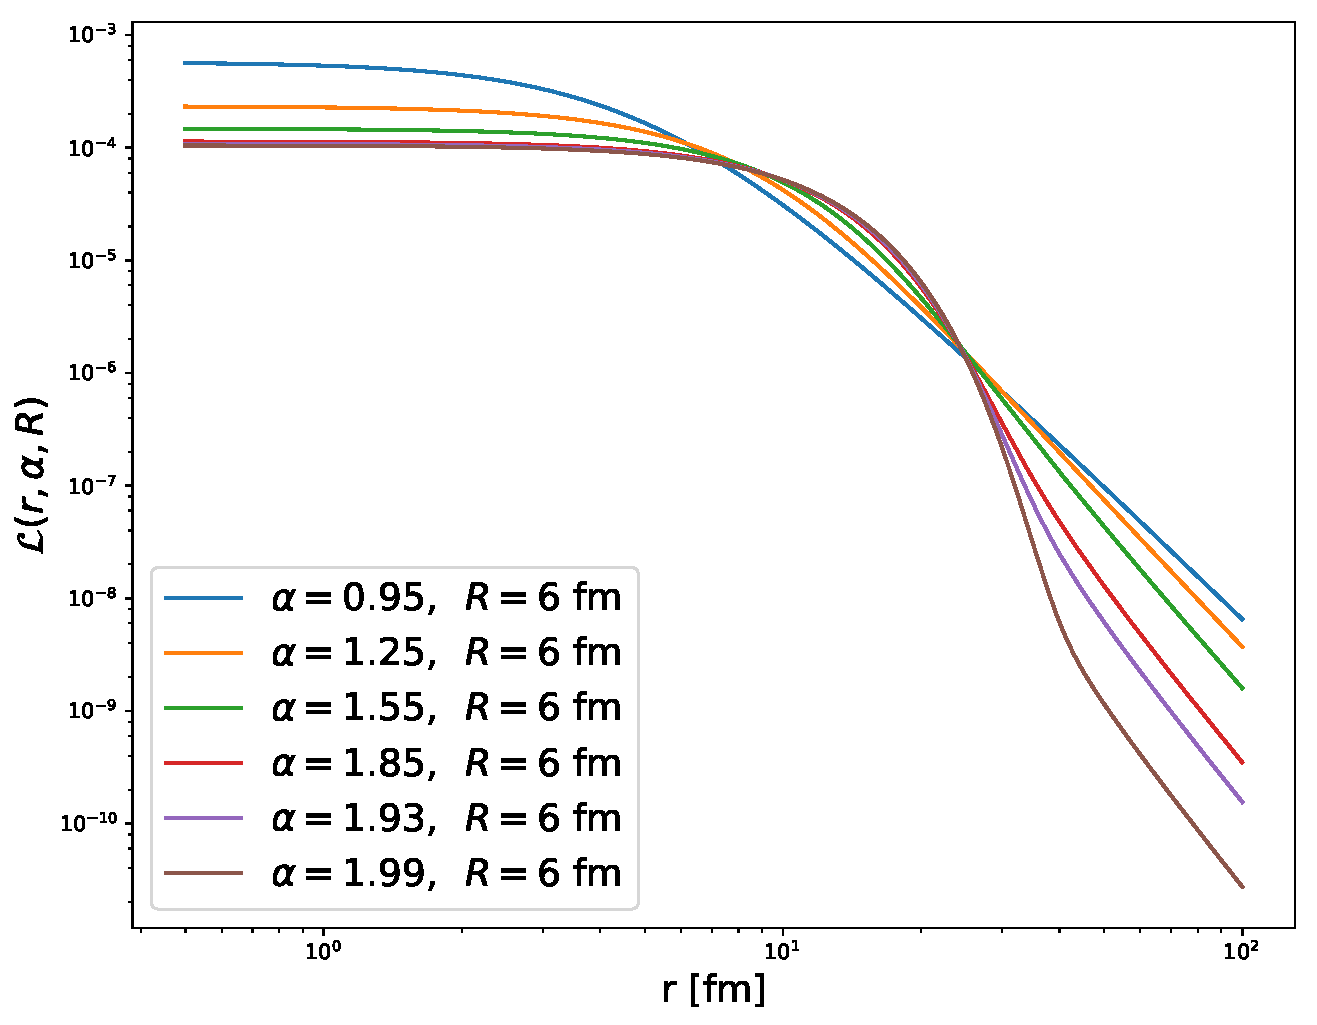
\includegraphics[scale=0.35]{pic/Coulomb/Levy_alpha.pdf}
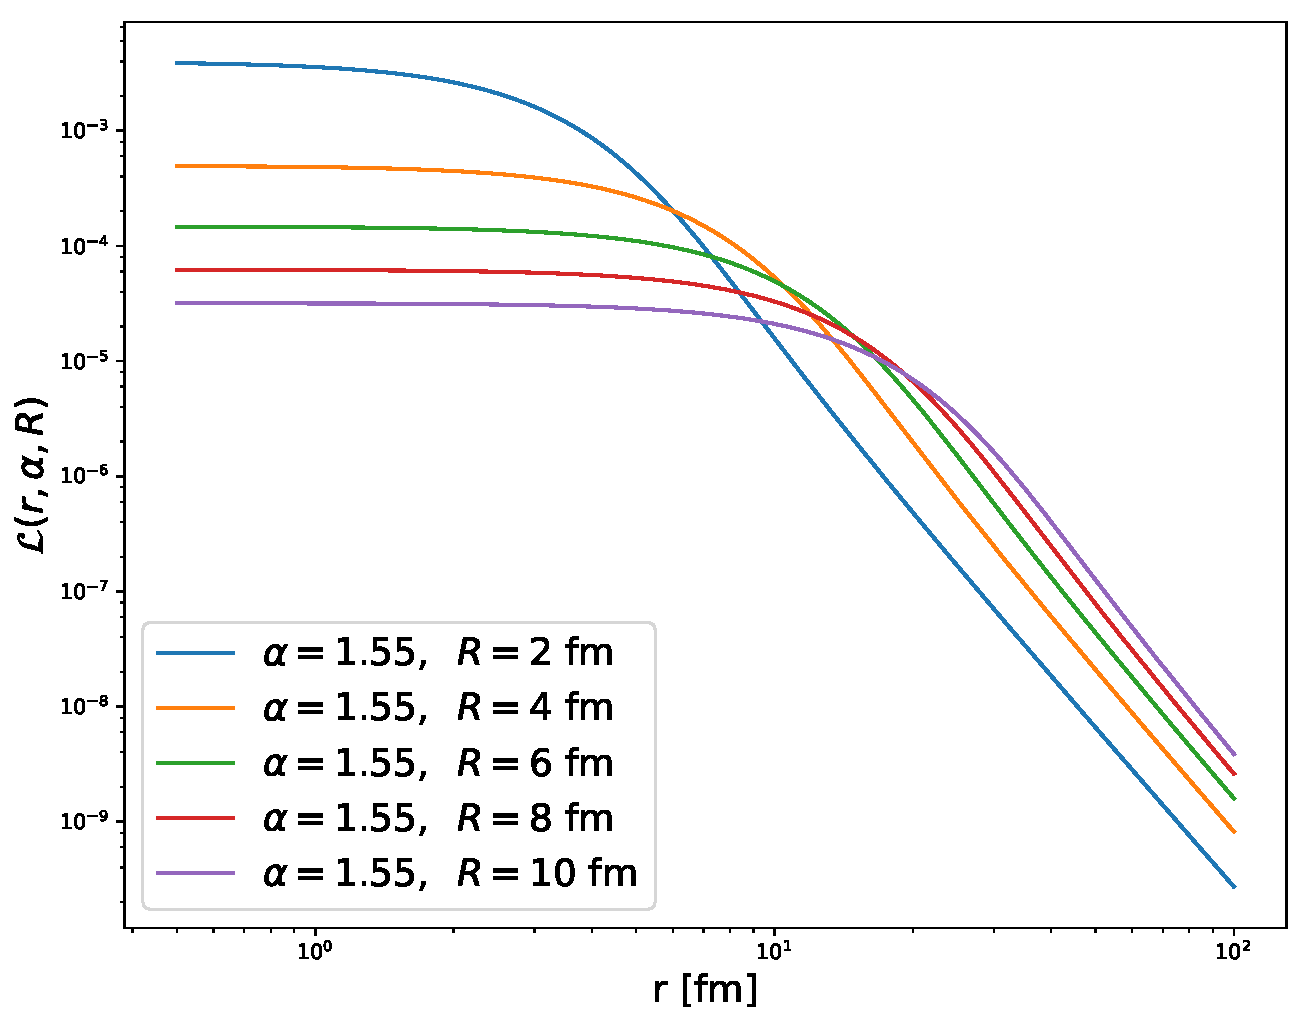
\includegraphics[scale=0.35]{pic/Coulomb/Levy_R.pdf}
\caption{Háromdimenziós Lévy eloszlás sugárfüggése különböző $\alpha$ és $R$ paraméterek esetén.}
\label{fig:Levy}
\end{figure}

\subsection{A mag-glória modell}

\subsection{A korreláció erőssége}

\subsection{Parciális koherencia}
kappa3

\section{Coulomb-korrekció számítása}
Háromrészecske: ~\cite{Alt:1998nr}
\subsection{Coulomb-kölcsönhatás}
\subsubsection{Kétrészecske}
hipergeometrikus függvény
számolás, aszimptotikus sor, cachelés
\subsubsection{Háromrészecske}

\subsection{A Coulomb-korrekciós integrál}

\subsection{Adaptív Gauss–Kronrod módszer}\label{sec:GK}

\subsection{Markov chain Monte Carlo módszerek}
kézzel írott jegyzetet beírni
\subsection{Monte Carlo módszer}
\subsection{Markov lánc}
Markov tulajdonság, grafikus model, faktorizál

\subsection{Implementáció}
\subsubsection{CUDA}\label{sec:CUDA}
\subsubsection{MapReduce}\label{sec:MapReduce}

\begin{figure}[H]
\centering
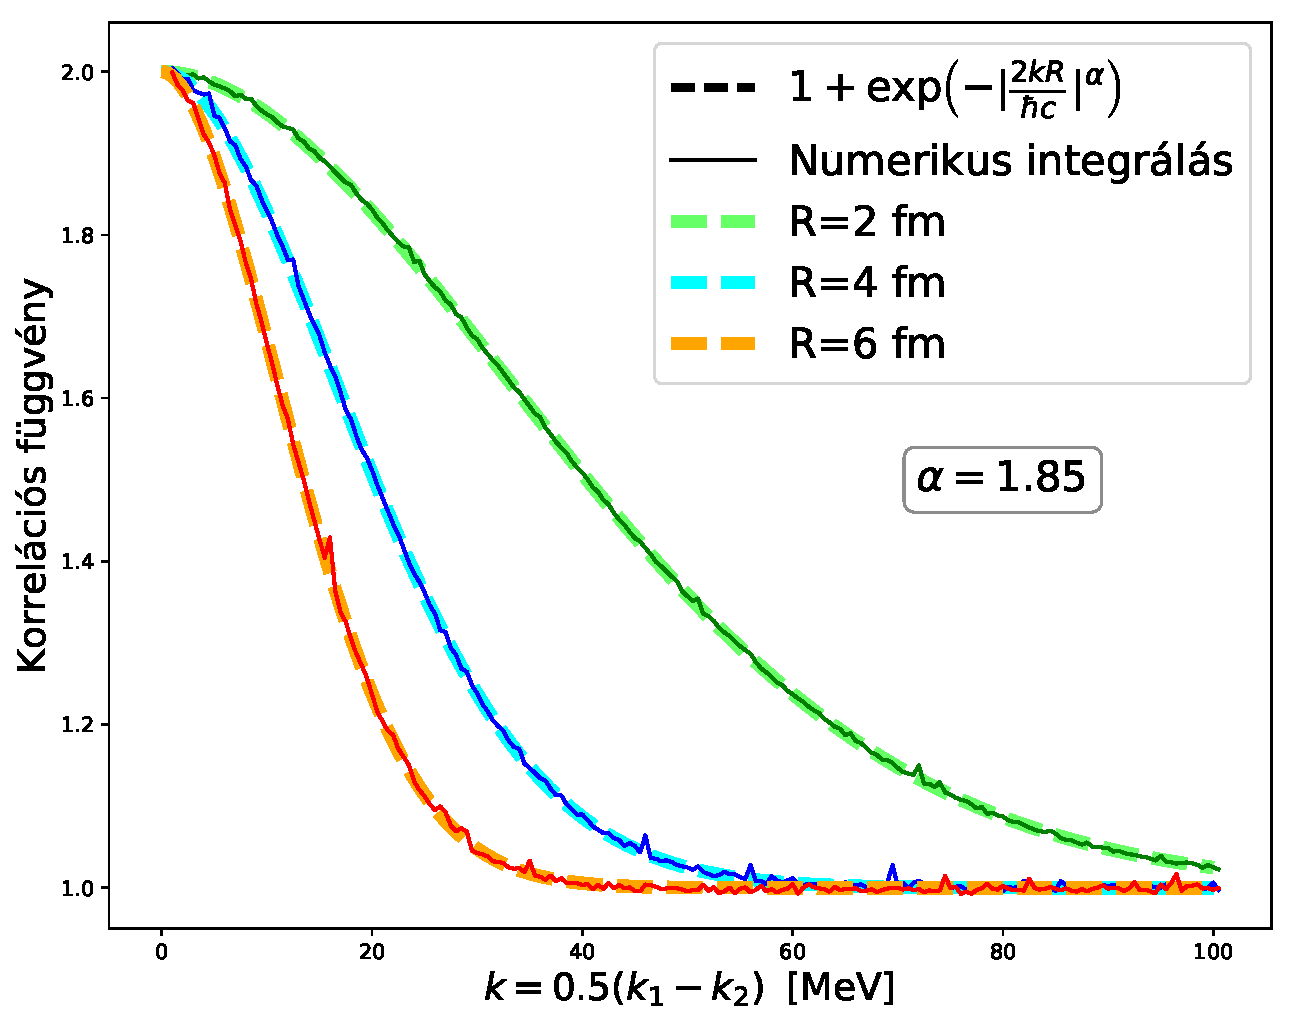
\includegraphics[scale=0.36]{pic/Coulomb/C2_noCoulomb_R246_a185.pdf}
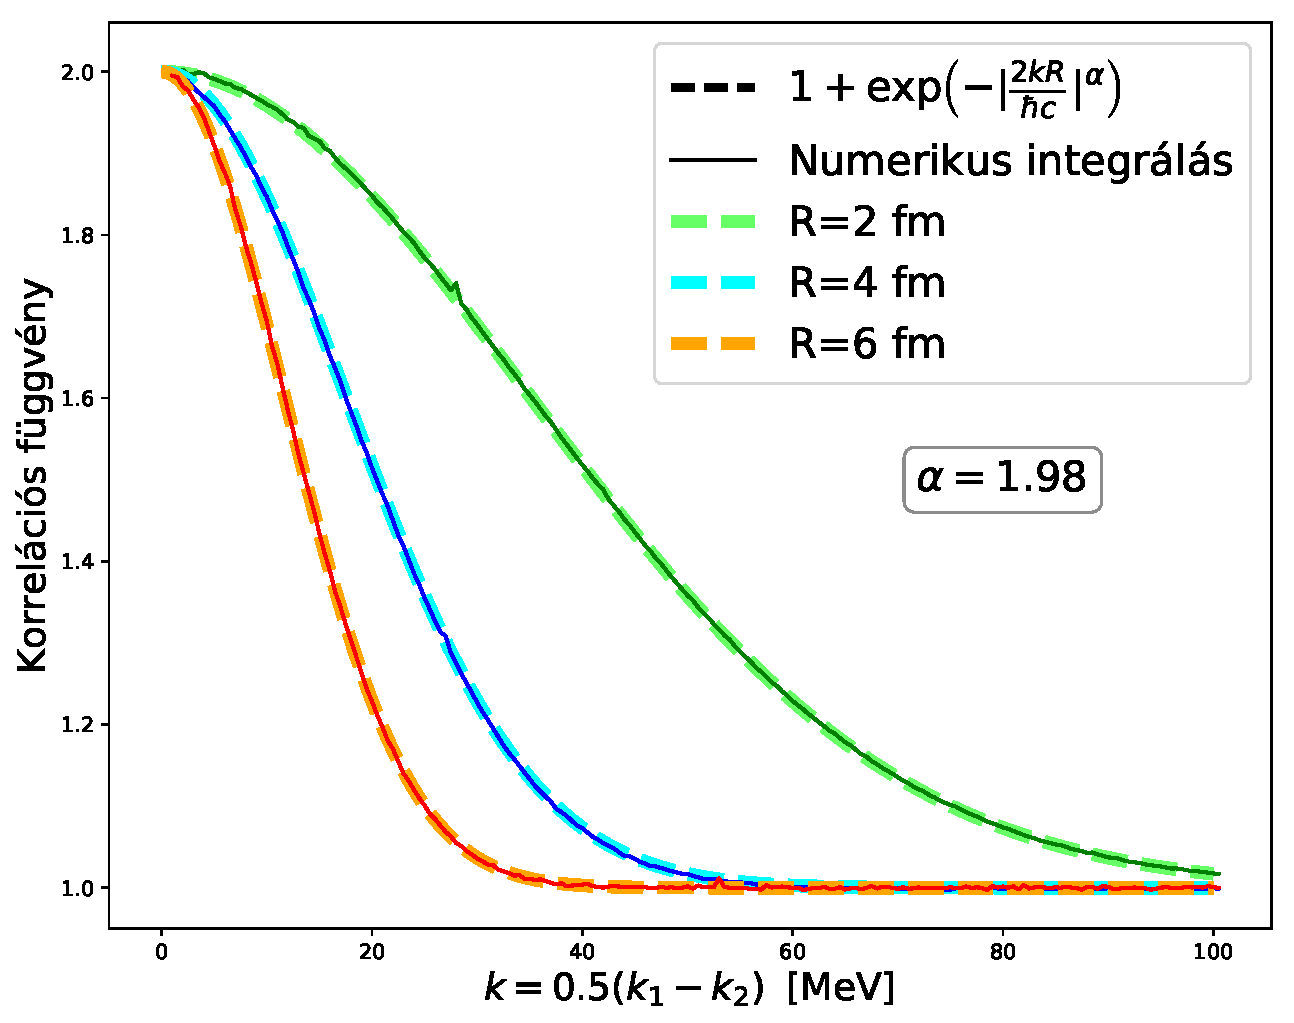
\includegraphics[scale=0.36]{pic/Coulomb/C2_noCoulomb_R246_a198.pdf}
\end{figure}

\begin{figure}[H]
\centering
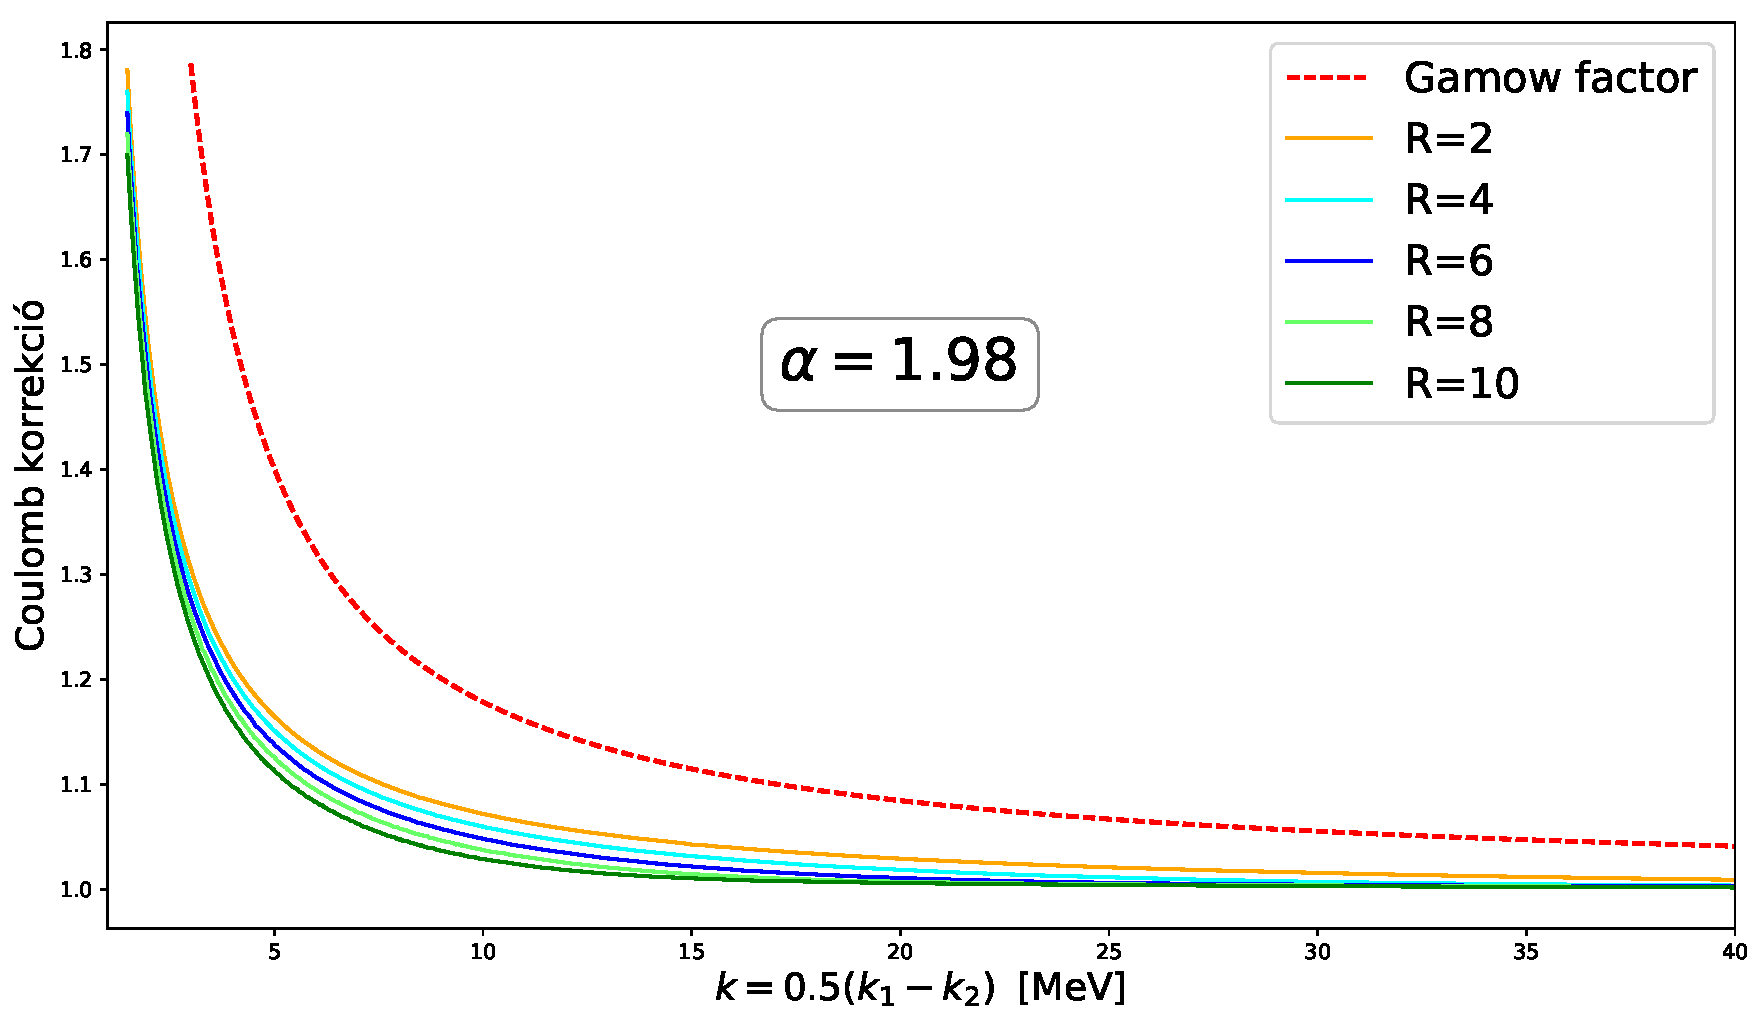
\includegraphics[scale=0.55]{pic/Coulomb/C2_R246810_a198.pdf}
\end{figure}


\section{Adatanalízis}
\subsection{Korrelációs függvény változói}
\subsection{Korrelációs függvény mérése}
\subsection{Illesztett modell}

\section{Eredmények}
\subsection{Illesztés vizualizáció}
\subsection{Háromrészecske korrelációs erősség}
\subsection{Parciális koherencia}


\section{Összefoglaló}




\bibliography{ref}

\end{document}
